% Options for packages loaded elsewhere
\PassOptionsToPackage{unicode}{hyperref}
\PassOptionsToPackage{hyphens}{url}
%
\documentclass[
]{article}
\usepackage{amsmath,amssymb}
\usepackage{lmodern}
\usepackage{iftex}
\ifPDFTeX
  \usepackage[T1]{fontenc}
  \usepackage[utf8]{inputenc}
  \usepackage{textcomp} % provide euro and other symbols
\else % if luatex or xetex
  \usepackage{unicode-math}
  \defaultfontfeatures{Scale=MatchLowercase}
  \defaultfontfeatures[\rmfamily]{Ligatures=TeX,Scale=1}
\fi
% Use upquote if available, for straight quotes in verbatim environments
\IfFileExists{upquote.sty}{\usepackage{upquote}}{}
\IfFileExists{microtype.sty}{% use microtype if available
  \usepackage[]{microtype}
  \UseMicrotypeSet[protrusion]{basicmath} % disable protrusion for tt fonts
}{}
\makeatletter
\@ifundefined{KOMAClassName}{% if non-KOMA class
  \IfFileExists{parskip.sty}{%
    \usepackage{parskip}
  }{% else
    \setlength{\parindent}{0pt}
    \setlength{\parskip}{6pt plus 2pt minus 1pt}}
}{% if KOMA class
  \KOMAoptions{parskip=half}}
\makeatother
\usepackage{xcolor}
\usepackage[margin=1in]{geometry}
\usepackage{color}
\usepackage{fancyvrb}
\newcommand{\VerbBar}{|}
\newcommand{\VERB}{\Verb[commandchars=\\\{\}]}
\DefineVerbatimEnvironment{Highlighting}{Verbatim}{commandchars=\\\{\}}
% Add ',fontsize=\small' for more characters per line
\usepackage{framed}
\definecolor{shadecolor}{RGB}{248,248,248}
\newenvironment{Shaded}{\begin{snugshade}}{\end{snugshade}}
\newcommand{\AlertTok}[1]{\textcolor[rgb]{0.94,0.16,0.16}{#1}}
\newcommand{\AnnotationTok}[1]{\textcolor[rgb]{0.56,0.35,0.01}{\textbf{\textit{#1}}}}
\newcommand{\AttributeTok}[1]{\textcolor[rgb]{0.77,0.63,0.00}{#1}}
\newcommand{\BaseNTok}[1]{\textcolor[rgb]{0.00,0.00,0.81}{#1}}
\newcommand{\BuiltInTok}[1]{#1}
\newcommand{\CharTok}[1]{\textcolor[rgb]{0.31,0.60,0.02}{#1}}
\newcommand{\CommentTok}[1]{\textcolor[rgb]{0.56,0.35,0.01}{\textit{#1}}}
\newcommand{\CommentVarTok}[1]{\textcolor[rgb]{0.56,0.35,0.01}{\textbf{\textit{#1}}}}
\newcommand{\ConstantTok}[1]{\textcolor[rgb]{0.00,0.00,0.00}{#1}}
\newcommand{\ControlFlowTok}[1]{\textcolor[rgb]{0.13,0.29,0.53}{\textbf{#1}}}
\newcommand{\DataTypeTok}[1]{\textcolor[rgb]{0.13,0.29,0.53}{#1}}
\newcommand{\DecValTok}[1]{\textcolor[rgb]{0.00,0.00,0.81}{#1}}
\newcommand{\DocumentationTok}[1]{\textcolor[rgb]{0.56,0.35,0.01}{\textbf{\textit{#1}}}}
\newcommand{\ErrorTok}[1]{\textcolor[rgb]{0.64,0.00,0.00}{\textbf{#1}}}
\newcommand{\ExtensionTok}[1]{#1}
\newcommand{\FloatTok}[1]{\textcolor[rgb]{0.00,0.00,0.81}{#1}}
\newcommand{\FunctionTok}[1]{\textcolor[rgb]{0.00,0.00,0.00}{#1}}
\newcommand{\ImportTok}[1]{#1}
\newcommand{\InformationTok}[1]{\textcolor[rgb]{0.56,0.35,0.01}{\textbf{\textit{#1}}}}
\newcommand{\KeywordTok}[1]{\textcolor[rgb]{0.13,0.29,0.53}{\textbf{#1}}}
\newcommand{\NormalTok}[1]{#1}
\newcommand{\OperatorTok}[1]{\textcolor[rgb]{0.81,0.36,0.00}{\textbf{#1}}}
\newcommand{\OtherTok}[1]{\textcolor[rgb]{0.56,0.35,0.01}{#1}}
\newcommand{\PreprocessorTok}[1]{\textcolor[rgb]{0.56,0.35,0.01}{\textit{#1}}}
\newcommand{\RegionMarkerTok}[1]{#1}
\newcommand{\SpecialCharTok}[1]{\textcolor[rgb]{0.00,0.00,0.00}{#1}}
\newcommand{\SpecialStringTok}[1]{\textcolor[rgb]{0.31,0.60,0.02}{#1}}
\newcommand{\StringTok}[1]{\textcolor[rgb]{0.31,0.60,0.02}{#1}}
\newcommand{\VariableTok}[1]{\textcolor[rgb]{0.00,0.00,0.00}{#1}}
\newcommand{\VerbatimStringTok}[1]{\textcolor[rgb]{0.31,0.60,0.02}{#1}}
\newcommand{\WarningTok}[1]{\textcolor[rgb]{0.56,0.35,0.01}{\textbf{\textit{#1}}}}
\usepackage{longtable,booktabs,array}
\usepackage{calc} % for calculating minipage widths
% Correct order of tables after \paragraph or \subparagraph
\usepackage{etoolbox}
\makeatletter
\patchcmd\longtable{\par}{\if@noskipsec\mbox{}\fi\par}{}{}
\makeatother
% Allow footnotes in longtable head/foot
\IfFileExists{footnotehyper.sty}{\usepackage{footnotehyper}}{\usepackage{footnote}}
\makesavenoteenv{longtable}
\usepackage{graphicx}
\makeatletter
\def\maxwidth{\ifdim\Gin@nat@width>\linewidth\linewidth\else\Gin@nat@width\fi}
\def\maxheight{\ifdim\Gin@nat@height>\textheight\textheight\else\Gin@nat@height\fi}
\makeatother
% Scale images if necessary, so that they will not overflow the page
% margins by default, and it is still possible to overwrite the defaults
% using explicit options in \includegraphics[width, height, ...]{}
\setkeys{Gin}{width=\maxwidth,height=\maxheight,keepaspectratio}
% Set default figure placement to htbp
\makeatletter
\def\fps@figure{htbp}
\makeatother
\setlength{\emergencystretch}{3em} % prevent overfull lines
\providecommand{\tightlist}{%
  \setlength{\itemsep}{0pt}\setlength{\parskip}{0pt}}
\setcounter{secnumdepth}{-\maxdimen} % remove section numbering
\ifLuaTeX
  \usepackage{selnolig}  % disable illegal ligatures
\fi
\IfFileExists{bookmark.sty}{\usepackage{bookmark}}{\usepackage{hyperref}}
\IfFileExists{xurl.sty}{\usepackage{xurl}}{} % add URL line breaks if available
\urlstyle{same} % disable monospaced font for URLs
\hypersetup{
  pdftitle={Labo 5: Paramètres de tendance centrale},
  pdfauthor={Visseho Adjiwanou, PhD.},
  hidelinks,
  pdfcreator={LaTeX via pandoc}}

\title{Labo 5: Paramètres de tendance centrale}
\author{Visseho Adjiwanou, PhD.}
\date{07 February 2023}

\begin{document}
\maketitle

\hypertarget{partie-a}{%
\section{PARTIE A}\label{partie-a}}

\hypertarget{question-1-tiruxe9-de-krieg}{%
\subsection{Question 1: (tiré de
Krieg)}\label{question-1-tiruxe9-de-krieg}}

A partir des données du tableau suivant, calculer :

\begin{itemize}
\tightlist
\item
  le mode
\item
  la médiane
\item
  la moyenne
\item
  l'étendue
\item
  l'écart inter-quartile
\item
  la variance et l'écart-type
\end{itemize}

\begin{longtable}[]{@{}lllll@{}}
\toprule()
NE & Fréquence & Pourcentage & Pourcentage valide & Pourcentage
cumulé \\
\midrule()
\endhead
0 & 414 & 28.1 & 28.1 & 28.1 \\
1 & 242 & 16.4 & 16.4 & 44.5 \\
2 & 398 & 27.0 & 27.0 & 71.4 \\
3 & 226 & 15.3 & 15.3 & 86.8 \\
4 & 115 & 7.8 & 7.8 & 94.6 \\
5 & 58 & 3.9 & 3.9 & 98.6 \\
6 & 14 & .9 & .9 & 99.5 \\
7 & 7 & .5 & .5 & 100.0 \\
\bottomrule()
\end{longtable}

NE : Nombre d'enfants

\textbf{Taille de l'échantillon} N = 414 + 242 + \ldots{} + 7

\textbf{Niveau de mesure de la variable}

Ratio

\hypertarget{ruxe9ponse}{%
\subsubsection{Réponse}\label{ruxe9ponse}}

\begin{itemize}
\item
  Mode : 0
\item
  Médiane : 44,5\% des répondants ont au plus 1 enfant (c'est à dire
  qu'ils en ont 0 ou 1). 71,4\% ont au plus 2 enfants (c'est à dire
  qu'ils en ont 0, ou 1 ou 2). Donc, on peut dire que la moitié de
  l'échantillon (50\%) a entre 1 et 2 enfants. La médiane est alors
  l'intervalle {[}1,2{]}. On peut être plus précis en utilisant la
  formule de la fois passée:
\end{itemize}

1 médiane 2 44.5\% 50\% 71.4 414+242=656 1474/2=737 414+242+398=1054

(Médiane - 2)/(50 - 71.4) = (1 - 2)/(44.5 - 71.4)

Médiane = 2 + (1-2)/(44.5 - 71.4)*(50 - 71.4)

Médiane = 1.2 enfants

Autre manière de le visualiser: On a au total 1474 répondants. La moitié
est entre 737 et 737.5

0 1 md 2 414 242 737 398 658 1056

737 est plus proche de 658 (donc de 1) que de 1056 (2)

(mediane - 2)/(737 - 1056) = (1-2)/(658-1056) mediane = 2 +
(1-2)/(658-1056)*(737 - 1056) mediane = 1.20

\begin{itemize}
\tightlist
\item
  Moyenne
\end{itemize}

\begin{longtable}[]{@{}lllll@{}}
\toprule()
NE & Fréquence & Pourcentage & Pourcentage valide & Pourcentage
cumulé \\
\midrule()
\endhead
0 & 414 & 28.1 & 28.1 & 28.1 \\
1 & 242 & 16.4 & 16.4 & 44.5 \\
2 & 398 & 27.0 & 27.0 & 71.4 \\
3 & 226 & 15.3 & 15.3 & 86.8 \\
4 & 115 & 7.8 & 7.8 & 94.6 \\
5 & 58 & 3.9 & 3.9 & 98.6 \\
6 & 14 & .9 & .9 & 99.5 \\
7 & 7 & .5 & .5 & 100.0 \\
\bottomrule()
\end{longtable}

\begin{Shaded}
\begin{Highlighting}[]
\DecValTok{414}\SpecialCharTok{*}\DecValTok{0} \SpecialCharTok{+} \DecValTok{242}\SpecialCharTok{*}\DecValTok{1} \SpecialCharTok{+} \DecValTok{298}\SpecialCharTok{*}\DecValTok{2} \SpecialCharTok{+} \DecValTok{226}\SpecialCharTok{*}\DecValTok{3} \SpecialCharTok{+} \DecValTok{115}\SpecialCharTok{*}\DecValTok{4} \SpecialCharTok{+} \DecValTok{58}\SpecialCharTok{*}\DecValTok{5} \SpecialCharTok{+} \DecValTok{14}\SpecialCharTok{*}\DecValTok{6} \SpecialCharTok{+} \DecValTok{7}\SpecialCharTok{*}\DecValTok{7}
\end{Highlighting}
\end{Shaded}

\begin{verbatim}
## [1] 2399
\end{verbatim}

\begin{Shaded}
\begin{Highlighting}[]
\DecValTok{414} \SpecialCharTok{+} \DecValTok{242} \SpecialCharTok{+} \DecValTok{398} \SpecialCharTok{+} \DecValTok{226} \SpecialCharTok{+} \DecValTok{115} \SpecialCharTok{+} \DecValTok{58} \SpecialCharTok{+} \DecValTok{14} \SpecialCharTok{+}\DecValTok{7}
\end{Highlighting}
\end{Shaded}

\begin{verbatim}
## [1] 1474
\end{verbatim}

\begin{Shaded}
\begin{Highlighting}[]
\NormalTok{moyenne }\OtherTok{\textless{}{-}} \DecValTok{2399} \SpecialCharTok{/} \DecValTok{1474}
\NormalTok{moyenne }
\end{Highlighting}
\end{Shaded}

\begin{verbatim}
## [1] 1.627544
\end{verbatim}

mode \textless{} médiane \textless{} moyenne ==\textgreater{}
asymétrique avec un étalement vers la droite.

\hypertarget{parametres-de-dispersion}{%
\section{Parametres de dispersion}\label{parametres-de-dispersion}}

\begin{itemize}
\item
  étendue : 7 - 0 = 7 enfants
\item
  EIQ:

  \begin{itemize}
  \tightlist
  \item
    1e Quartile : 25\% des gens ont 0 enfant donc 1eQ = 0
  \end{itemize}
\end{itemize}

2 3eq 3\\
71.4 75\% 86.8\%

3eq = 3 + (2-3)/(71.4 - 86.8)*(75 - 86.8) = 2.2

\begin{itemize}
\tightlist
\item
  3e quartile: 75\% des gens ont entre 2 et 3 enfants = 2.2
\end{itemize}

donc EIQ = 2.2 - 0 = 2.2

Exemple simple pour calculer le Q1, Q2 et l'écart:

\url{https://www150.statcan.gc.ca/n1/edu/power-pouvoir/ch12/5214890-fra.htm\#}:\textasciitilde:text=L'\%C3\%A9cart\%20interquartile\%20est\%20une,comme\%20mesure\%20de\%20la\%20dispersion.\&text=L'\%C3\%A9cart\%20interquartile\%20couvre\%2050,le\%20quartile\%20le\%20plus\%20faible.

\begin{itemize}
\tightlist
\item
  Variance
\end{itemize}

\begin{longtable}[]{@{}lllll@{}}
\toprule()
NE & Fréquence & Pourcentage & Pourcentage valide & Pourcentage
cumulé \\
\midrule()
\endhead
0 & 414 & 28.1 & 28.1 & 28.1 \\
1 & 242 & 16.4 & 16.4 & 44.5 \\
2 & 398 & 27.0 & 27.0 & 71.4 \\
3 & 226 & 15.3 & 15.3 & 86.8 \\
4 & 115 & 7.8 & 7.8 & 94.6 \\
5 & 58 & 3.9 & 3.9 & 98.6 \\
6 & 14 & .9 & .9 & 99.5 \\
7 & 7 & .5 & .5 & 100.0 \\
\bottomrule()
\end{longtable}

La formule de la varianlce est \(\frac{\sum(X_i - \bar{X})^2}{N-1}\)

414 personnes avec 0 enfant

\begin{Shaded}
\begin{Highlighting}[]
\CommentTok{\# A = (0 {-} 1.6)\^{}2 + ... + (0 {-} 1.6)\^{}2, 414 fois}

\NormalTok{A }\OtherTok{\textless{}{-}} \DecValTok{414}\SpecialCharTok{*}\NormalTok{(}\DecValTok{0}\FloatTok{{-}1.6}\NormalTok{)}\SpecialCharTok{\^{}}\DecValTok{2}
\NormalTok{B}\OtherTok{\textless{}{-}} \DecValTok{242}\SpecialCharTok{*}\NormalTok{(}\DecValTok{1} \SpecialCharTok{{-}} \FloatTok{1.6}\NormalTok{)}\SpecialCharTok{\^{}}\DecValTok{2}
\NormalTok{C }\OtherTok{\textless{}{-}} \DecValTok{398}\SpecialCharTok{*}\NormalTok{(}\DecValTok{2} \SpecialCharTok{{-}} \FloatTok{1.6}\NormalTok{)}\SpecialCharTok{\^{}}\DecValTok{2}
\NormalTok{D }\OtherTok{\textless{}{-}} \DecValTok{226}\SpecialCharTok{*}\NormalTok{(}\DecValTok{3} \SpecialCharTok{{-}}\FloatTok{1.6}\NormalTok{)}\SpecialCharTok{\^{}}\DecValTok{2}
\NormalTok{E }\OtherTok{\textless{}{-}} \DecValTok{115}\SpecialCharTok{*}\NormalTok{(}\DecValTok{4} \SpecialCharTok{{-}} \FloatTok{1.6}\NormalTok{)}\SpecialCharTok{\^{}}\DecValTok{2}
\NormalTok{F }\OtherTok{\textless{}{-}} \DecValTok{58}\SpecialCharTok{*}\NormalTok{(}\DecValTok{5} \SpecialCharTok{{-}} \FloatTok{1.6}\NormalTok{)}\SpecialCharTok{\^{}}\DecValTok{2}
\NormalTok{G }\OtherTok{\textless{}{-}} \DecValTok{14}\SpecialCharTok{*}\NormalTok{(}\DecValTok{6} \SpecialCharTok{{-}} \FloatTok{1.6}\NormalTok{)}\SpecialCharTok{\^{}}\DecValTok{2}
\NormalTok{H }\OtherTok{\textless{}{-}} \DecValTok{7}\SpecialCharTok{*}\NormalTok{(}\DecValTok{7} \SpecialCharTok{{-}} \FloatTok{1.6}\NormalTok{)}\SpecialCharTok{\^{}}\DecValTok{2}

\NormalTok{somme }\OtherTok{\textless{}{-}}\NormalTok{ A }\SpecialCharTok{+}\NormalTok{ B }\SpecialCharTok{+}\NormalTok{ C }\SpecialCharTok{+}\NormalTok{ D }\SpecialCharTok{+}\NormalTok{ E }\SpecialCharTok{+}\NormalTok{ F }\SpecialCharTok{+}\NormalTok{ G }\SpecialCharTok{+}\NormalTok{ H}

\NormalTok{variance }\OtherTok{\textless{}{-}}\NormalTok{ somme }\SpecialCharTok{/}\NormalTok{ (}\DecValTok{1474} \SpecialCharTok{{-}}\DecValTok{1}\NormalTok{)}
\end{Highlighting}
\end{Shaded}

\begin{itemize}
\tightlist
\item
  écart-type
\end{itemize}

\begin{Shaded}
\begin{Highlighting}[]
\NormalTok{ écart\_type }\OtherTok{\textless{}{-}} \FunctionTok{sqrt}\NormalTok{(variance)}
\end{Highlighting}
\end{Shaded}

\hypertarget{question-2-tiruxe9-de-krieg}{%
\subsection{Question 2: (tiré de
Krieg)}\label{question-2-tiruxe9-de-krieg}}

Le graphique suivant présente l'histogramme de l'âge au premier mariage.

\begin{figure}
\centering
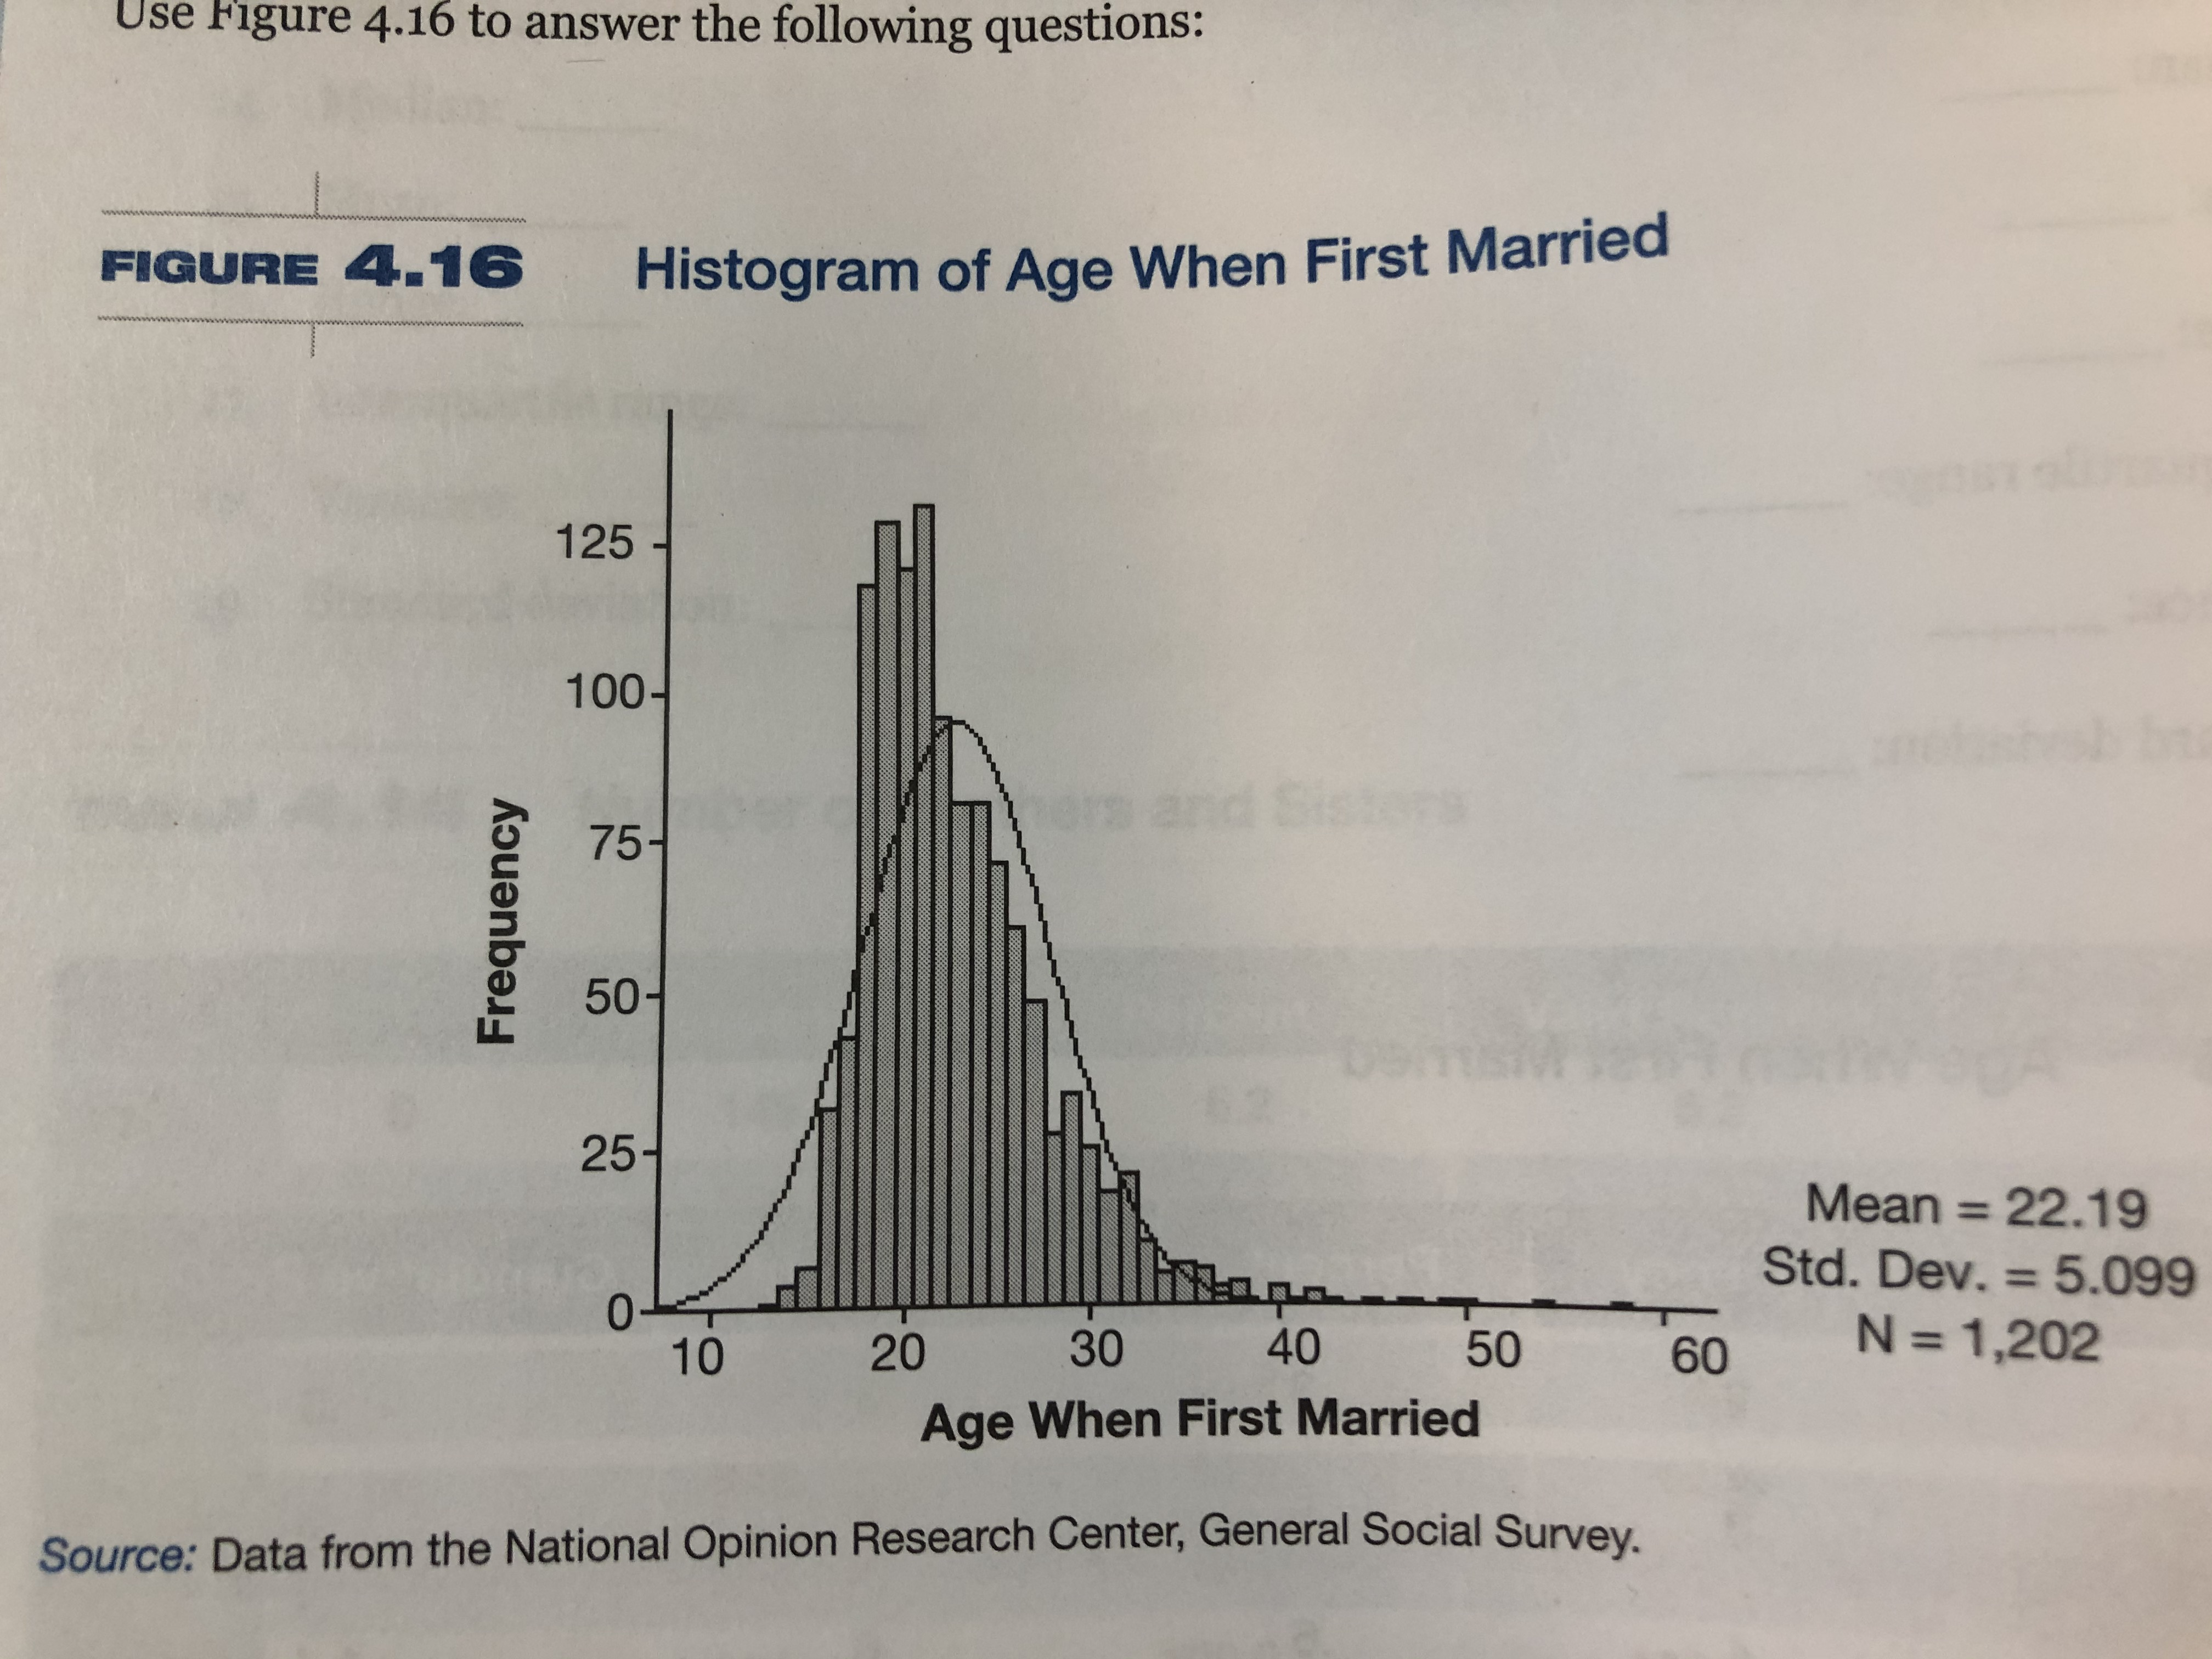
\includegraphics{Histogramme_age_mariage.jpg}
\caption{Figure 1: Histogramme de l'âge au premier mariage}
\end{figure}

A partir de ce graphique, répondez aux questions suivantes:

\begin{enumerate}
\def\labelenumi{\arabic{enumi}.}
\tightlist
\item
  Quel est l'âge moyen des répondant.es à leur premier mariage?
\end{enumerate}

22.19

\begin{enumerate}
\def\labelenumi{\arabic{enumi}.}
\setcounter{enumi}{1}
\item
  Combien de répondant.es ont été enquêté.es? 1202
\item
  Quelle est la valeur de la variance?
\end{enumerate}

\begin{Shaded}
\begin{Highlighting}[]
\NormalTok{variance }\OtherTok{\textless{}{-}} \FloatTok{5.099}\SpecialCharTok{\^{}}\DecValTok{2}
\end{Highlighting}
\end{Shaded}

\begin{enumerate}
\def\labelenumi{\arabic{enumi}.}
\setcounter{enumi}{3}
\item
  En se basant sur les propriétés de la courbe normale, nous pouvons
  dire que 68\% des répondant.es se sont marié.es entre les âges 22.19 -
  5.099 et 22.19 + 5.099, soit entre 17.10 et 27.29 ans.
\item
  En se basant sur les propriétés de la courbe normale, nous pouvons
  dire que 95\% des répondant.es se sont marié.es entre les âges
  \texttt{22.19\ -\ 2*5.099} et \texttt{22.19\ +\ 2*5.099} soit entre
  12.00 ans et 32.38 ans
\end{enumerate}

\hypertarget{question-4---repruxe9sentation-graphique}{%
\subsection{Question 4 - représentation
graphique}\label{question-4---repruxe9sentation-graphique}}

Quelles sont les types de représentation graphique que l'on peut faire
avec une variable quantitative (ratio ou intervalle) ?

\begin{itemize}
\tightlist
\item
  \textbf{Histogramme. l'histogramme est différent d'un diagramme de
  barre}
\item
  \textbf{Diagramme de quartile encore appelé ``boîte à moustache''}
\end{itemize}

\hypertarget{exemple-du-cours}{%
\subsection{Exemple du cours}\label{exemple-du-cours}}

\begin{Shaded}
\begin{Highlighting}[]
\NormalTok{Score }\OtherTok{\textless{}{-}} \FunctionTok{c}\NormalTok{(}\DecValTok{64}\NormalTok{, }\DecValTok{68}\NormalTok{, }\DecValTok{70}\NormalTok{, }\DecValTok{71}\NormalTok{, }\DecValTok{69}\NormalTok{, }\DecValTok{66}\NormalTok{)}
\NormalTok{Score}
\end{Highlighting}
\end{Shaded}

\begin{verbatim}
## [1] 64 68 70 71 69 66
\end{verbatim}

\begin{Shaded}
\begin{Highlighting}[]
\NormalTok{Z\_score }\OtherTok{\textless{}{-}}\NormalTok{ (Score }\SpecialCharTok{{-}} \FunctionTok{mean}\NormalTok{(Score))}\SpecialCharTok{/}\FunctionTok{sd}\NormalTok{(Score)}
\NormalTok{Z\_score}
\end{Highlighting}
\end{Shaded}

\begin{verbatim}
## [1] -1.5339300  0.0000000  0.7669650  1.1504475  0.3834825 -0.7669650
\end{verbatim}

\begin{Shaded}
\begin{Highlighting}[]
\CommentTok{\# Moyenne}
\FunctionTok{mean}\NormalTok{(Z\_score)}
\end{Highlighting}
\end{Shaded}

\begin{verbatim}
## [1] 0
\end{verbatim}

\begin{Shaded}
\begin{Highlighting}[]
\CommentTok{\# Écart{-}type}
\FunctionTok{sd}\NormalTok{(Z\_score)}
\end{Highlighting}
\end{Shaded}

\begin{verbatim}
## [1] 1
\end{verbatim}

\hypertarget{partie-b}{%
\section{PARTIE B}\label{partie-b}}

\hypertarget{la-solution-technologique-au-changement-climatique-suite-et-fin-exemple-tiruxe9-de-krieg}{%
\section{La solution technologique au changement climatique, suite et
fin (exemple tiré de
Krieg)}\label{la-solution-technologique-au-changement-climatique-suite-et-fin-exemple-tiruxe9-de-krieg}}

À partir de la base d données que vous avez crées et utilisées à partir
des données sur les voitures, répondez aux questions suivantes en
utilisant R:

\begin{itemize}
\tightlist
\item
  Pour 1994
\end{itemize}

\begin{Shaded}
\begin{Highlighting}[]
\CommentTok{\# Créons d\textquotesingle{}abord des vecteurs}

\NormalTok{marque\_1994 }\OtherTok{\textless{}{-}} \FunctionTok{c}\NormalTok{(}\StringTok{"Mazda 626"}\NormalTok{, }\StringTok{"Honda Accord"}\NormalTok{, }\StringTok{"Chevrolet Corsica"}\NormalTok{, }\StringTok{"Buick Century"}\NormalTok{, }\StringTok{"Oldsmobile Cutlass Ciera"}\NormalTok{, }\StringTok{"Oldsmobile Achieva"}\NormalTok{, }\StringTok{"Pontiac Grand Am"}\NormalTok{, }\StringTok{"Infiniti G20"}\NormalTok{, }\StringTok{"Mitsubishi Galant"}\NormalTok{, }\StringTok{"Dodge Spirit"}\NormalTok{, }\StringTok{"Plymouth Acclaim"}\NormalTok{, }\StringTok{"Subaru Legacy"}\NormalTok{, }\StringTok{"Toyota Camry"}\NormalTok{, }\StringTok{"Hyundai Sonata"}\NormalTok{, }\StringTok{"Chrysler LeBaron"}\NormalTok{, }\StringTok{"Ford Taurus"}\NormalTok{, }\StringTok{"Mercury Sable"}\NormalTok{, }\StringTok{"Eagle Vision"}\NormalTok{)}
\NormalTok{marque\_1994}
\end{Highlighting}
\end{Shaded}

\begin{verbatim}
##  [1] "Mazda 626"                "Honda Accord"            
##  [3] "Chevrolet Corsica"        "Buick Century"           
##  [5] "Oldsmobile Cutlass Ciera" "Oldsmobile Achieva"      
##  [7] "Pontiac Grand Am"         "Infiniti G20"            
##  [9] "Mitsubishi Galant"        "Dodge Spirit"            
## [11] "Plymouth Acclaim"         "Subaru Legacy"           
## [13] "Toyota Camry"             "Hyundai Sonata"          
## [15] "Chrysler LeBaron"         "Ford Taurus"             
## [17] "Mercury Sable"            "Eagle Vision"
\end{verbatim}

\begin{Shaded}
\begin{Highlighting}[]
\NormalTok{annee\_pas\_cool\_1994 }\OtherTok{\textless{}{-}} \FunctionTok{c}\NormalTok{(}\DecValTok{1994}\NormalTok{, }\DecValTok{1994}\NormalTok{, }\DecValTok{1994}\NormalTok{,}\DecValTok{1994}\NormalTok{, }\DecValTok{1994}\NormalTok{, }\DecValTok{1994}\NormalTok{, }\DecValTok{1994}\NormalTok{, }\DecValTok{1994}\NormalTok{, }\DecValTok{1994}\NormalTok{, }\DecValTok{1994}\NormalTok{, }\DecValTok{1994}\NormalTok{, }\DecValTok{1994}\NormalTok{, }\DecValTok{1994}\NormalTok{, }\DecValTok{1994}\NormalTok{, }\DecValTok{1994}\NormalTok{, }\DecValTok{1994}\NormalTok{, }\DecValTok{1994}\NormalTok{, }\DecValTok{1994}\NormalTok{)}
\NormalTok{annee\_pas\_cool\_1994}
\end{Highlighting}
\end{Shaded}

\begin{verbatim}
##  [1] 1994 1994 1994 1994 1994 1994 1994 1994 1994 1994 1994 1994 1994 1994 1994
## [16] 1994 1994 1994
\end{verbatim}

\begin{Shaded}
\begin{Highlighting}[]
\FunctionTok{length}\NormalTok{(marque\_1994)}
\end{Highlighting}
\end{Shaded}

\begin{verbatim}
## [1] 18
\end{verbatim}

\begin{Shaded}
\begin{Highlighting}[]
\NormalTok{annee\_un\_peu\_bon\_1994 }\OtherTok{\textless{}{-}} \FunctionTok{c}\NormalTok{(}\FunctionTok{rep}\NormalTok{(}\DecValTok{1994}\NormalTok{, }\DecValTok{18}\NormalTok{))  }\CommentTok{\# Que fait la fonction rep?}
\NormalTok{annee\_un\_peu\_bon\_1994}
\end{Highlighting}
\end{Shaded}

\begin{verbatim}
##  [1] 1994 1994 1994 1994 1994 1994 1994 1994 1994 1994 1994 1994 1994 1994 1994
## [16] 1994 1994 1994
\end{verbatim}

\begin{Shaded}
\begin{Highlighting}[]
\NormalTok{annee\_1994 }\OtherTok{\textless{}{-}} \FunctionTok{c}\NormalTok{(}\FunctionTok{rep}\NormalTok{(}\DecValTok{1994}\NormalTok{, }\FunctionTok{length}\NormalTok{(marque\_1994))) }\CommentTok{\# que fait la fonction length?}

\NormalTok{annee\_1994}
\end{Highlighting}
\end{Shaded}

\begin{verbatim}
##  [1] 1994 1994 1994 1994 1994 1994 1994 1994 1994 1994 1994 1994 1994 1994 1994
## [16] 1994 1994 1994
\end{verbatim}

\begin{Shaded}
\begin{Highlighting}[]
\NormalTok{mpg\_ville\_1994 }\OtherTok{\textless{}{-}} \FunctionTok{c}\NormalTok{(}\DecValTok{23}\NormalTok{, }\FunctionTok{rep}\NormalTok{(}\DecValTok{22}\NormalTok{, }\DecValTok{4}\NormalTok{), }\FunctionTok{rep}\NormalTok{(}\DecValTok{21}\NormalTok{, }\DecValTok{6}\NormalTok{), }\FunctionTok{rep}\NormalTok{(}\DecValTok{20}\NormalTok{, }\DecValTok{2}\NormalTok{), }\FunctionTok{rep}\NormalTok{(}\DecValTok{19}\NormalTok{, }\DecValTok{2}\NormalTok{), }\FunctionTok{rep}\NormalTok{(}\DecValTok{18}\NormalTok{, }\DecValTok{3}\NormalTok{))}
\NormalTok{mpg\_ville\_1994}
\end{Highlighting}
\end{Shaded}

\begin{verbatim}
##  [1] 23 22 22 22 22 21 21 21 21 21 21 20 20 19 19 18 18 18
\end{verbatim}

\begin{Shaded}
\begin{Highlighting}[]
\NormalTok{mpg\_autoroute\_1994 }\OtherTok{\textless{}{-}} \FunctionTok{c}\NormalTok{(}\DecValTok{31}\NormalTok{, }\DecValTok{29}\NormalTok{, }\FunctionTok{rep}\NormalTok{(}\DecValTok{28}\NormalTok{, }\DecValTok{3}\NormalTok{), }\FunctionTok{rep}\NormalTok{(}\DecValTok{32}\NormalTok{, }\DecValTok{2}\NormalTok{), }\DecValTok{29}\NormalTok{, }\DecValTok{28}\NormalTok{, }\FunctionTok{rep}\NormalTok{(}\DecValTok{27}\NormalTok{, }\DecValTok{2}\NormalTok{), }\DecValTok{28}\NormalTok{, }\DecValTok{27}\NormalTok{, }\DecValTok{26}\NormalTok{, }\DecValTok{25}\NormalTok{, }\FunctionTok{rep}\NormalTok{(}\DecValTok{27}\NormalTok{, }\DecValTok{2}\NormalTok{), }\DecValTok{26}\NormalTok{)}
\NormalTok{mpg\_autoroute\_1994}
\end{Highlighting}
\end{Shaded}

\begin{verbatim}
##  [1] 31 29 28 28 28 32 32 29 28 27 27 28 27 26 25 27 27 26
\end{verbatim}

Une fois qu'on a créé les vecteurs, on peut facilement créer les deux
bases de données

\begin{Shaded}
\begin{Highlighting}[]
\NormalTok{donnee\_1994 }\OtherTok{\textless{}{-}} \FunctionTok{data.frame}\NormalTok{(}\AttributeTok{marque =}\NormalTok{ marque\_1994, }\AttributeTok{annee =}\NormalTok{ annee\_1994, }\AttributeTok{vitesse\_ville =}\NormalTok{ mpg\_ville\_1994, }\AttributeTok{vitesse\_autoroute =}\NormalTok{ mpg\_autoroute\_1994)}

\NormalTok{donnee\_1994}
\end{Highlighting}
\end{Shaded}

\begin{verbatim}
##                      marque annee vitesse_ville vitesse_autoroute
## 1                 Mazda 626  1994            23                31
## 2              Honda Accord  1994            22                29
## 3         Chevrolet Corsica  1994            22                28
## 4             Buick Century  1994            22                28
## 5  Oldsmobile Cutlass Ciera  1994            22                28
## 6        Oldsmobile Achieva  1994            21                32
## 7          Pontiac Grand Am  1994            21                32
## 8              Infiniti G20  1994            21                29
## 9         Mitsubishi Galant  1994            21                28
## 10             Dodge Spirit  1994            21                27
## 11         Plymouth Acclaim  1994            21                27
## 12            Subaru Legacy  1994            20                28
## 13             Toyota Camry  1994            20                27
## 14           Hyundai Sonata  1994            19                26
## 15         Chrysler LeBaron  1994            19                25
## 16              Ford Taurus  1994            18                27
## 17            Mercury Sable  1994            18                27
## 18             Eagle Vision  1994            18                26
\end{verbatim}

Maintenant, on peut le sauvegarder si on veut pour ne pas être amené à
refaire tout cela la prochaine fois. Remarquer que je l'ai enrégistré
comme un fichier R (extension .RDS)

\begin{Shaded}
\begin{Highlighting}[]
\FunctionTok{saveRDS}\NormalTok{(donnee\_1994, }\StringTok{"donnee1994.RDS"}\NormalTok{)}
\end{Highlighting}
\end{Shaded}

Je peux alors l'ouvrir et l'utiliser

\begin{Shaded}
\begin{Highlighting}[]
\NormalTok{d1994 }\OtherTok{\textless{}{-}} \FunctionTok{readRDS}\NormalTok{(}\StringTok{"donnee1994.RDS"}\NormalTok{)  }\CommentTok{\# Que signifie d1994?}
\end{Highlighting}
\end{Shaded}

\begin{enumerate}
\def\labelenumi{\arabic{enumi}.}
\tightlist
\item
  Recalculer les paramètres de position sur les variables suivantes:
\end{enumerate}

\begin{itemize}
\tightlist
\item
  la vitesse en ville en 1994
\item
  la vitesse sur autoroute en 1994
\item
  la vitesse en ville en 2009
\item
  la vitesse sur autoroute en 2009
\end{itemize}

Je calcule la moyenne et la médiane pour les variables vitesse sur
autorute et en ville en 1994.

\begin{Shaded}
\begin{Highlighting}[]
\CommentTok{\# Moyenne}

\NormalTok{moyenne\_vitesse\_ville\_1994 }\OtherTok{\textless{}{-}} \FunctionTok{mean}\NormalTok{(d1994}\SpecialCharTok{$}\NormalTok{vitesse\_ville)}
\NormalTok{moyenne\_vitesse\_ville\_1994}
\end{Highlighting}
\end{Shaded}

\begin{verbatim}
## [1] 20.5
\end{verbatim}

\begin{Shaded}
\begin{Highlighting}[]
\NormalTok{moyenne\_vitesse\_autoroute\_1994 }\OtherTok{\textless{}{-}} \FunctionTok{mean}\NormalTok{(d1994}\SpecialCharTok{$}\NormalTok{vitesse\_autoroute)}
\NormalTok{moyenne\_vitesse\_autoroute\_1994}
\end{Highlighting}
\end{Shaded}

\begin{verbatim}
## [1] 28.05556
\end{verbatim}

\begin{Shaded}
\begin{Highlighting}[]
  \CommentTok{\# Mis dans le même vecteur}
\NormalTok{moy\_ville\_autoroute\_1994 }\OtherTok{\textless{}{-}} \FunctionTok{c}\NormalTok{(moyenne\_vitesse\_ville\_1994, moyenne\_vitesse\_autoroute\_1994)}
\NormalTok{moy\_ville\_autoroute\_1994}
\end{Highlighting}
\end{Shaded}

\begin{verbatim}
## [1] 20.50000 28.05556
\end{verbatim}

\begin{Shaded}
\begin{Highlighting}[]
\CommentTok{\#Mediane}

\NormalTok{mediane\_vitesse\_ville\_1994 }\OtherTok{\textless{}{-}} \FunctionTok{median}\NormalTok{(d1994}\SpecialCharTok{$}\NormalTok{vitesse\_ville)}
\NormalTok{mediane\_vitesse\_ville\_1994}
\end{Highlighting}
\end{Shaded}

\begin{verbatim}
## [1] 21
\end{verbatim}

\begin{Shaded}
\begin{Highlighting}[]
\NormalTok{mediane\_vitesse\_autoroute\_1994 }\OtherTok{\textless{}{-}} \FunctionTok{median}\NormalTok{(d1994}\SpecialCharTok{$}\NormalTok{vitesse\_autoroute)}
\NormalTok{mediane\_vitesse\_autoroute\_1994}
\end{Highlighting}
\end{Shaded}

\begin{verbatim}
## [1] 28
\end{verbatim}

\begin{Shaded}
\begin{Highlighting}[]
  \CommentTok{\# Mis dans le même vecteur}
\NormalTok{med\_ville\_autoroute\_1994 }\OtherTok{\textless{}{-}} \FunctionTok{c}\NormalTok{(mediane\_vitesse\_ville\_1994, mediane\_vitesse\_autoroute\_1994)}
\NormalTok{med\_ville\_autoroute\_1994}
\end{Highlighting}
\end{Shaded}

\begin{verbatim}
## [1] 21 28
\end{verbatim}

\begin{Shaded}
\begin{Highlighting}[]
\CommentTok{\# Mis ensemble dans un fichier}

\NormalTok{lieu }\OtherTok{\textless{}{-}} \FunctionTok{c}\NormalTok{(}\StringTok{"Ville"}\NormalTok{, }\StringTok{"Autoroute"}\NormalTok{)}

\NormalTok{Tendance\_1994 }\OtherTok{\textless{}{-}} \FunctionTok{data.frame}\NormalTok{(lieu, moy\_ville\_autoroute\_1994, med\_ville\_autoroute\_1994)}
\NormalTok{Tendance\_1994}
\end{Highlighting}
\end{Shaded}

\begin{verbatim}
##        lieu moy_ville_autoroute_1994 med_ville_autoroute_1994
## 1     Ville                 20.50000                       21
## 2 Autoroute                 28.05556                       28
\end{verbatim}

\hypertarget{interpruxe9tation-des-ruxe9sultats}{%
\subsubsection{Interprétation des
résultats}\label{interpruxe9tation-des-ruxe9sultats}}

On voit que qu'en moyenne, la vitesse est en moyenne plus grande sur
l'autoroute qu'en ville. Les moyennes sont très proches des médianes.

\begin{enumerate}
\def\labelenumi{\arabic{enumi}.}
\setcounter{enumi}{1}
\tightlist
\item
  Calculer la variance et l'écart-type des quatre variables précédentes.
\end{enumerate}

\begin{Shaded}
\begin{Highlighting}[]
\CommentTok{\# Variance}
\NormalTok{variance\_vitesse\_ville\_1994 }\OtherTok{\textless{}{-}} \FunctionTok{var}\NormalTok{(d1994}\SpecialCharTok{$}\NormalTok{vitesse\_ville)}
\NormalTok{variance\_vitesse\_ville\_1994}
\end{Highlighting}
\end{Shaded}

\begin{verbatim}
## [1] 2.382353
\end{verbatim}

\begin{Shaded}
\begin{Highlighting}[]
\NormalTok{variance\_vitesse\_autoroute\_1994 }\OtherTok{\textless{}{-}} \FunctionTok{var}\NormalTok{(d1994}\SpecialCharTok{$}\NormalTok{vitesse\_autoroute)}
\NormalTok{variance\_vitesse\_autoroute\_1994}
\end{Highlighting}
\end{Shaded}

\begin{verbatim}
## [1] 3.820261
\end{verbatim}

\begin{Shaded}
\begin{Highlighting}[]
\NormalTok{var\_1994 }\OtherTok{\textless{}{-}} \FunctionTok{c}\NormalTok{(variance\_vitesse\_ville\_1994, variance\_vitesse\_autoroute\_1994)}

\CommentTok{\# Écart{-}type}


\NormalTok{ecart\_type\_vitesse\_ville\_1994 }\OtherTok{\textless{}{-}} \FunctionTok{sd}\NormalTok{(d1994}\SpecialCharTok{$}\NormalTok{vitesse\_ville)}
\NormalTok{ecart\_type\_vitesse\_ville\_1994}
\end{Highlighting}
\end{Shaded}

\begin{verbatim}
## [1] 1.543487
\end{verbatim}

\begin{Shaded}
\begin{Highlighting}[]
\NormalTok{ecart\_type\_vitesse\_autoroute\_1994 }\OtherTok{\textless{}{-}} \FunctionTok{sd}\NormalTok{(d1994}\SpecialCharTok{$}\NormalTok{vitesse\_autoroute)}
\NormalTok{ecart\_type\_vitesse\_autoroute\_1994}
\end{Highlighting}
\end{Shaded}

\begin{verbatim}
## [1] 1.954549
\end{verbatim}

\begin{Shaded}
\begin{Highlighting}[]
\NormalTok{ecart\_1994 }\OtherTok{\textless{}{-}} \FunctionTok{c}\NormalTok{(ecart\_type\_vitesse\_ville\_1994, ecart\_type\_vitesse\_autoroute\_1994)}

\NormalTok{Variation\_1994 }\OtherTok{\textless{}{-}} \FunctionTok{data.frame}\NormalTok{(lieu, var\_1994, ecart\_1994)}
\NormalTok{Variation\_1994}
\end{Highlighting}
\end{Shaded}

\begin{verbatim}
##        lieu var_1994 ecart_1994
## 1     Ville 2.382353   1.543487
## 2 Autoroute 3.820261   1.954549
\end{verbatim}

\begin{enumerate}
\def\labelenumi{\arabic{enumi}.}
\setcounter{enumi}{2}
\tightlist
\item
  Comment ces résultats permettent-ils d'infirmer ou de renforcer la
  conclusion que vous avez tiré sur la solution technologique au
  changement climatique tiré au 1.
\end{enumerate}

Pour répondre à cette question, j'ai besoin des données de 2009. Je vous
laisse donc créer cette seconde base de données à partir des données du
tableau du labo 4 et répondre à l'ensemble des questions. Bon travail.

\hypertarget{solution-de-la-question-4}{%
\subsection{Solution de la question 4}\label{solution-de-la-question-4}}

laissez-moi vous entraîner dans la passion des statistiques.

\begin{enumerate}
\def\labelenumi{\arabic{enumi}.}
\setcounter{enumi}{4}
\tightlist
\item
  La distribution d'échantillonnage n'est rien d'autre que la
  distribution d'un échantillon (Vrai ou Faux)
\end{enumerate}

Réponse: Faux.

Une distribution d'échantillonnage correspond à une distribution de
statistiques quelconques (moyennes, médianes, etc.) provenant de tous
les échantillons possibles d'une taille donnée que l'on peut tirer d'une
population déterminée. Une distribution d'un échantillon est la
distribution des scores à l'intérieur d'un échantillon d'une taille
donnée.

Voici une manière de comprendre la distribution d'échantillon. On va
utiliser les données du marathon de Boston de 2012. Le tableau présente
la description de cette base de données:

\begin{longtable}[]{@{}ll@{}}
\toprule()
Variables & Description \\
\midrule()
\endhead
V1 & Nom \\
V2 & Sexe \\
V3 & Age \\
V4 & Division \\
V5 & Pays \\
V6 & Temps mis \\
\bottomrule()
\end{longtable}

Pour estimer le temps moyen que ce marathon a été couru, nous n'avons
pas besoin d'avoir forcément l'ensemble des résultats de la course. Un
échantillon représentatif devrait suffire à nous fournir ce résultat.
Donc, nous allons prendre un échantillon de 40 coureurs et calculer le
temps moyen mis. Pour le moment, nous vivons comme si nous ne
connaissons par le temps vrai (issu de la course).

Nous chargeons la base de données dans R.

\begin{Shaded}
\begin{Highlighting}[]
\FunctionTok{rm}\NormalTok{(}\AttributeTok{list =} \FunctionTok{ls}\NormalTok{())}
\NormalTok{marathon }\OtherTok{\textless{}{-}} \FunctionTok{read.csv}\NormalTok{(}\StringTok{"bm\_results2012.txt"}\NormalTok{, }\AttributeTok{header =} \ConstantTok{FALSE}\NormalTok{, }\AttributeTok{quote =} \StringTok{""}\NormalTok{)}
\end{Highlighting}
\end{Shaded}

On voit ainsi que 21541 personnes ont couru ce marathon.

Pour tirer un échantillon, nous allons utiliser la fonction
\textbf{sample\_n} du package \textbf{dplyr}. Comme toujours, vous devez
installer ce package (une seule fois), le charger (avant toute
utilisation).

\begin{Shaded}
\begin{Highlighting}[]
\CommentTok{\#install.packages("dplyr")}
\FunctionTok{library}\NormalTok{(tidyverse)}
\end{Highlighting}
\end{Shaded}

\begin{verbatim}
## -- Attaching packages --------------------------------------- tidyverse 1.3.2 --
## v ggplot2 3.3.6     v purrr   0.3.4
## v tibble  3.1.6     v dplyr   1.0.8
## v tidyr   1.2.0     v stringr 1.4.1
## v readr   2.1.2     v forcats 0.5.2
\end{verbatim}

\begin{verbatim}
## Warning: package 'tibble' was built under R version 3.6.2
\end{verbatim}

\begin{verbatim}
## Warning: package 'tidyr' was built under R version 3.6.2
\end{verbatim}

\begin{verbatim}
## Warning: package 'readr' was built under R version 3.6.2
\end{verbatim}

\begin{verbatim}
## Warning: package 'purrr' was built under R version 3.6.2
\end{verbatim}

\begin{verbatim}
## Warning: package 'dplyr' was built under R version 3.6.2
\end{verbatim}

\begin{verbatim}
## -- Conflicts ------------------------------------------ tidyverse_conflicts() --
## x dplyr::filter() masks stats::filter()
## x dplyr::lag()    masks stats::lag()
\end{verbatim}

\begin{Shaded}
\begin{Highlighting}[]
\FunctionTok{set.seed}\NormalTok{(}\DecValTok{430}\NormalTok{)}
\NormalTok{marathon\_S1 }\OtherTok{\textless{}{-}} \FunctionTok{sample\_n}\NormalTok{(marathon, }\DecValTok{40}\NormalTok{, }\AttributeTok{replace =} \ConstantTok{FALSE}\NormalTok{)}
\end{Highlighting}
\end{Shaded}

Nous voyons ainsi que marathon\_S1 a juste 40 observations.

\textbf{Remarques:}

\begin{enumerate}
\def\labelenumi{\arabic{enumi}.}
\tightlist
\item
  dplyr fait partie d'une famille de package qui s'appelle
  \textbf{tidyverse} que nous allons voir lors du prochain cours.
\item
  L'option replace = FALSE signifie que quand nous tirons un élément de
  la population, nous ne le retournons pas dans la population avant de
  tirer le second.
\item
  Même si on choisit les individus de manières aléatoires, on veut quand
  même que d'autres personnes tirent exactement les mêmes individus que
  nous s'ils veulent vérifier nos résultats. set.seed(n'importe quel
  chiffre) permet de tirer chaque fois le même échantillon. N'utiliser
  pas cela quand vous faites vos calculs, cela va nous permettre de voir
  les différents résultats que nous obtenons tous.
\item
  Un rappel sur l'échantillonage :
  \url{https://www150.statcan.gc.ca/n1/edu/power-pouvoir/ch13/prob/5214899-fra.htm}
\end{enumerate}

Ainsi, à partir de notre échantillon tiré, on peut calculer le temps
moyen mis pour courir le marathon de

1, 2, 3, NA 1, 2, 3

\begin{Shaded}
\begin{Highlighting}[]
\NormalTok{temps\_moyen\_S1 }\OtherTok{\textless{}{-}} \FunctionTok{mean}\NormalTok{(marathon\_S1}\SpecialCharTok{$}\NormalTok{V6, }\AttributeTok{na.rm =} \ConstantTok{TRUE}\NormalTok{)}
\NormalTok{temps\_moyen\_S1}
\end{Highlighting}
\end{Shaded}

\begin{verbatim}
## [1] 268.5303
\end{verbatim}

\begin{Shaded}
\begin{Highlighting}[]
\FunctionTok{sd}\NormalTok{(marathon\_S1}\SpecialCharTok{$}\NormalTok{V6)}
\end{Highlighting}
\end{Shaded}

\begin{verbatim}
## [1] 45.23583
\end{verbatim}

268 +- 1.96*ecart-type/racine carré(N)

On voit ainsi qu'à partir de notre échantillon que le temps mis pour
parcourir le marathon de New York est de 268.5 minutes.

Maintenant, jetons un coup d'œil sur les vrais résultats de ce marathon.

\begin{Shaded}
\begin{Highlighting}[]
\NormalTok{temps\_moyen\_vrai }\OtherTok{\textless{}{-}} \FunctionTok{mean}\NormalTok{(marathon}\SpecialCharTok{$}\NormalTok{V6, }\AttributeTok{na.rm =} \ConstantTok{TRUE}\NormalTok{)}
\NormalTok{temps\_moyen\_vrai}
\end{Highlighting}
\end{Shaded}

\begin{verbatim}
## [1] 263.0493
\end{verbatim}

Le temps moyen mis en vrai est de 263.0 minutes. Voyez comment est
proche notre estimation à partir juste d'un échantillon aléatoire de 40
coureur.es.

Voua avez tous obtenus une réponse différente de la mienne. Une
distribution d'échantillonnage n'est rien d'autre que l'ensemble des
moyennes qu'on peut calculer à partir des millions d'échantillon de
taille 40 de cette population de 21541 coureurs. En fait, on connaît
exactement le nombre d'échantillons possible qu'on peut tirer. C'est
cela qui s'appelle une combinaison avec la formule
\(C_{21541}^{40} =\frac{21541!}{40!(21541 - 40)!}\). Tenez-vous bien, ce
nombre équivaut à :

253
077729093757612460294630785205954107797288308598032063927991250054643573537874160223994161945109975602007594
059 581 835 406 976

\{A, B, C, D\}

:\{A, B\}, \{A, C\}

J'ai utilisé ce générateur en ligne pour le calculer :
\url{https://www.dcode.fr/combinaisons}

Bref, revenons à notre exercice. Aujourd'hui avec la puissance des
machine, on peut déterminer en une fraction de secondes le nombre total
d'échantillon. Mais, au fait, si on peut tirer tous ces échantillons,
n'est-il juste pas plus simple de collecter l'information sur l'ensemble
de la population ? Bien sûr. Dans les faits, on ne tirera jamais plus
d'un échantillon.

Si je prenais par contre 100 échantillons de taille 40, la distribution
que j'obtiens de la moyenne est ce qu'on appelle \textbf{une
distribution d'échantillonnage}. Voyons ce que cela donne :

\begin{Shaded}
\begin{Highlighting}[]
\FunctionTok{set.seed}\NormalTok{(}\DecValTok{123432}\NormalTok{)}

\NormalTok{marat\_T40\_R100 }\OtherTok{\textless{}{-}} \FunctionTok{bind\_rows}\NormalTok{(}\FunctionTok{replicate}\NormalTok{(}\DecValTok{100}\NormalTok{, }\FunctionTok{sample\_n}\NormalTok{(marathon, }\DecValTok{40}\NormalTok{, }\AttributeTok{replace =} \ConstantTok{FALSE}\NormalTok{), }\AttributeTok{simplify =}\NormalTok{ F), }\AttributeTok{.id =} \StringTok{"Obs"}\NormalTok{)}
\end{Highlighting}
\end{Shaded}

En lisant cette syntaxe de la droite vers la gauche, cela veut dire que
: - \textbf{sample\_n(marathon, 40, replace = FALSE), simplify = F)}: je
tire un échantillon de taille 40 dans la base de données
\textbf{marathon} - \textbf{(replicate(100, sample\_n(marathon, 40,
replace = FALSE)} : je replique cela 100 fois; -
\textbf{bind\_rows(replicate(100, sample\_n(marathon, 40, replace =
FALSE), simplify = F), .id = ``Obs'')}: Je les colle ensemble (avec la
fonction bind\_rows de dplyr) en les distinguant par leur numéro dans la
nouvelle variable ``Obs''

C'est tout. Vous voyez que cela me donne un échantillon de 4000
observations. La variable Obs distingue ainsi chaque unique échantillon.

Si nous calculons alors la moyenne de chaque échantillon on obtient la
base de données avec les moyenne. On va utiliser la fonction stby de
summarytools pour faire cela facilement. Remarquez une fois de plus que
je charge ce package avant de l'utiliser.

\begin{Shaded}
\begin{Highlighting}[]
\CommentTok{\#library(summarytools)}

\CommentTok{\#with(marat\_T40\_R100, stby(data = V6, INDICES = Obs,}
\CommentTok{\#     FUN = descr, stats = c("mean")))}
\end{Highlighting}
\end{Shaded}

Summarytools ne semble pas fonctionner, je vais utiliser une autre
option:

\begin{Shaded}
\begin{Highlighting}[]
\NormalTok{Moyenne\_T40\_R100 }\OtherTok{\textless{}{-}}
\NormalTok{  marat\_T40\_R100 }\SpecialCharTok{\%\textgreater{}\%} 
  \FunctionTok{group\_by}\NormalTok{(Obs) }\SpecialCharTok{\%\textgreater{}\%} 
  \FunctionTok{summarise}\NormalTok{(}\AttributeTok{moyenne =} \FunctionTok{mean}\NormalTok{(V6, }\AttributeTok{na.rm =} \ConstantTok{TRUE}\NormalTok{)) }

\NormalTok{Moyenne\_T40\_R100}
\end{Highlighting}
\end{Shaded}

\begin{verbatim}
## # A tibble: 100 x 2
##    Obs   moyenne
##    <chr>   <dbl>
##  1 1        259.
##  2 10       253.
##  3 100      265.
##  4 11       259.
##  5 12       267.
##  6 13       267.
##  7 14       271.
##  8 15       269.
##  9 16       255.
## 10 17       261.
## # ... with 90 more rows
\end{verbatim}

Ainsi, on a une nouvelle base de donnés avec les 100 moyennes issus de
chaque marathon échantillonné.

Dressons la distribution de ces 100 moyennes, à l'aide de l'histogramme

\begin{Shaded}
\begin{Highlighting}[]
\FunctionTok{hist}\NormalTok{(Moyenne\_T40\_R100}\SpecialCharTok{$}\NormalTok{moyenne)}
\end{Highlighting}
\end{Shaded}

\includegraphics{Labo5_Paramètres_variation_solution_détaillée_files/figure-latex/unnamed-chunk-19-1.pdf}

On voit ainsi que cela à l'allure d'une courbe normale.

Que pensez-vous que la moyenne de ces moyennes va nous donner?

\begin{Shaded}
\begin{Highlighting}[]
\NormalTok{moyenne\_moyenne }\OtherTok{\textless{}{-}} \FunctionTok{mean}\NormalTok{(Moyenne\_T40\_R100}\SpecialCharTok{$}\NormalTok{moyenne)}
\NormalTok{moyenne\_moyenne}
\end{Highlighting}
\end{Shaded}

\begin{verbatim}
## [1] 263.0335
\end{verbatim}

Cela nous donne exactement 263 minutes, ce qui est exactement la vraie
moyenne à quelque centième de seconde près. Bingo, la moyenne des
moyennes nous donne une estimation de la moyenne de la population.

Pour faire cet exercice, voici un peu toutes les recherches que j'ai
faites sur le net:


\includegraphics{recherche_net.png}

\begin{itemize}
\tightlist
\item
\end{itemize}

\begin{enumerate}
\def\labelenumi{\arabic{enumi}.}
\setcounter{enumi}{5}
\tightlist
\item
  Énoncez et expliquer le théorème de la \textbf{limite centrale}
\end{enumerate}

Ce théorème dit simplement que si N devient de plus en plus grand, la
forme de la courbe tend de plus en plus vers une courbe normale. Voyons
cela: A la place de 40 observations - Tirons plutôt 90; - Tirons à
nouveau 100 échantillons; - Calculons la vitesse moyenne de chaque
échantillon - Présentons l'histogramme de cette distribution

Vous pouvez le faire non? Essayer.

\begin{Shaded}
\begin{Highlighting}[]
\CommentTok{\# Echantillon}
\FunctionTok{set.seed}\NormalTok{(}\DecValTok{12343}\NormalTok{)}
\NormalTok{marat\_T90\_R100 }\OtherTok{\textless{}{-}} \FunctionTok{bind\_rows}\NormalTok{(}\FunctionTok{replicate}\NormalTok{(}\DecValTok{100}\NormalTok{, }\FunctionTok{sample\_n}\NormalTok{(marathon, }\DecValTok{90}\NormalTok{, }\AttributeTok{replace =} \ConstantTok{FALSE}\NormalTok{), }\AttributeTok{simplify =}\NormalTok{ F), }\AttributeTok{.id =} \StringTok{"Obs"}\NormalTok{)}

\CommentTok{\# Moyenne}

\NormalTok{Moyenne\_T90\_R100 }\OtherTok{\textless{}{-}}
\NormalTok{  marat\_T90\_R100 }\SpecialCharTok{\%\textgreater{}\%} 
  \FunctionTok{group\_by}\NormalTok{(Obs) }\SpecialCharTok{\%\textgreater{}\%} 
  \FunctionTok{summarise}\NormalTok{(}\AttributeTok{moyenne =} \FunctionTok{mean}\NormalTok{(V6, }\AttributeTok{na.rm =} \ConstantTok{TRUE}\NormalTok{))}

\CommentTok{\# Histogramme}

\FunctionTok{hist}\NormalTok{(Moyenne\_T40\_R100}\SpecialCharTok{$}\NormalTok{moyenne)}
\end{Highlighting}
\end{Shaded}

\includegraphics{Labo5_Paramètres_variation_solution_détaillée_files/figure-latex/unnamed-chunk-21-1.pdf}

et la moyenne des moyennes vaut

\begin{Shaded}
\begin{Highlighting}[]
\FunctionTok{mean}\NormalTok{(Moyenne\_T90\_R100}\SpecialCharTok{$}\NormalTok{moyenne)}
\end{Highlighting}
\end{Shaded}

\begin{verbatim}
## [1] 262.8977
\end{verbatim}

Vous verrez surtout que l'écart-type est plus faible.

\begin{Shaded}
\begin{Highlighting}[]
\FunctionTok{sd}\NormalTok{(Moyenne\_T90\_R100}\SpecialCharTok{$}\NormalTok{moyenne)}
\end{Highlighting}
\end{Shaded}

\begin{verbatim}
## [1] 5.428166
\end{verbatim}

Alors que avec l'échantillon de 40, cela donnait:

\begin{Shaded}
\begin{Highlighting}[]
\FunctionTok{sd}\NormalTok{(Moyenne\_T40\_R100}\SpecialCharTok{$}\NormalTok{moyenne)}
\end{Highlighting}
\end{Shaded}

\begin{verbatim}
## [1] 7.796008
\end{verbatim}

Quand la taille augmente, notre confiance dans les résultats augmente.

Alors, faites la même chose en choississant un échantillon de 150
coureur.es.

\begin{enumerate}
\def\labelenumi{\arabic{enumi}.}
\setcounter{enumi}{6}
\tightlist
\item
  Il n'y a pas de différence entre l'\textbf{écart-type} et
  l'\textbf{erreur-type}
\end{enumerate}

l'écart-type est ce que vous calculez à partir d'un seul échantillon,
alors que l'erreur-type est ce que vous calculez à partir d'une
distribution d'échantillonnage. Donc, en haut, j'ai plutôt calculé les
erreurs-types.

Pouvez-vous me dire alors, comment sont calculés les erreurs-type?

\textbf{N'est-ce pas formidable les statistiques?}

\end{document}
